\documentclass{../llncs2e/llncs}
\usepackage{inputenc}
\usepackage{graphicx}
\usepackage{caption}
% make a proper TOC despite llncs
\setcounter{tocdepth}{2}
\makeatletter
\renewcommand*\l@author[2]{}
\renewcommand*\l@title[2]{}
\makeatletter
\newcommand*\NewPage{\newpage\null\thispagestyle{empty}\newpage}
% page numbering
\pagestyle{plain}
% change the spacing between the caption and the table
\captionsetup[table]{skip=10pt}
% ------------------------------------------------------
% CLOUD OF THINGS DOCUMENT
% ------------------------------------------------------
\begin{document}
% ------------------------------------------------------
% MASTER THESIS PROJECT TITLE
% ------------------------------------------------------
\title{\vspace*{2in}\Huge Cloud4Things\vspace{2in}}
% ------------------------------------------------------
% AUTHOR
% ------------------------------------------------------
\author{\Large Marcus Vin\'icius Paulino Gomes}
% ------------------------------------------------------
% INSTITUTION
% ------------------------------------------------------
\institute{\large Instituto Superior T\'ecnico, Universidade de Lisboa\\
\email{marcus.paulino.gomes@tecnico.ulisboa.pt}}
\maketitle
\NewPage
\tableofcontents
\NewPage
\begin{abstract}
In this document we present Cloud4Things, a solution that proposes to make the deploy and manage IoT applications for smart places.
Due to the heterogeneity of IoT applications, management tasks such as application deployment and management are complex tasks
that require advanced technical knowledge. Cloud4Things proposes to decrease the complexity of these tasks by adopting a high-level perspective
enables to perform the deployment and management operations of IoT applications.
To simplify the deployment operation at the Cloud, Cloud4Things will rely on cloud orchestrators tools to execute such task.
These orchestration tools allow the specification of the application structure in high-level abstraction and allow the control the life-cycle of the application.
Cloud4Things will allow the management of the provisioned resources at the Cloud by a smart place only having in mind
the business rules of this particular space. With Cloud4Things, smart places managers will be able to monitor the performance of its
smart place in real time. This document also presents the state-of-the-art solution as well an overview about the proposed approaches and
evaluation methods.
\keywords{Internet of Things, Cloud Computing, Smart Places, Service Level Agreements, Orchestration Tools, Automated Deployment}
\end{abstract}

\NewPage
%!TEX root = ../dissertation.tex

\chapter{Introduction}
\label{chapter:introduction}
In recent years, computing is becoming more ubiquitous in the physical world. This notion where
computational elements are embedded seamlessly in ordinary objects that are connected through a
continuous network was introduced many years ago \cite{weiser1991computer}. The progress
towards ubiquitous computing has been slower than expected, technology advances such as the mobile
Internet contributes to achieve this vision in which computational devices are able to communicate
between themselves from any part of the world \cite{gubbi2013internet}. In this vision, an ubiquitous
system is composed of physical items that are continuously connected to the virtual world and can act as
remotely and physical access points to Internet Services \cite{mattern2010internet}.\\

However, there are some challenges that must be addressed in order to make these \gls{ubicomp} systems
truly ubiquitous \cite{caceres2012ubicomp}. An important concern regards about ubiquitous data: \textit{Where it is located?},
\textit{Who can access it?} and \textit{How much time this data should persist?}. Also, ubiquitous systems
are constantly interacting with the surrounding environment, thus these systems need to understand
the context in that they are inserted and also to adapt to the changes that occur in this environment.
Another import concern regards about the infrastructure burden of the ubiquitous systems. These
systems requires low-latency interaction with users and environments, which implies that at least part
of an \gls{ubicomp} application needs to be tightly bounded to the local infrastructure of the interacting
environment. This requirement for local infrastructure is a barrier in the adoption of ubiquitous
systems in a large-scale perspective.\\

This ubiquitous world is close to becoming reality thanks to the Utility Computing in the cloud
and the \gls{IoT}. In one hand, the utility computing provides the illusion of infinite computing
resources available on demand to the public users \cite{armbrust2010view}, which helps to reduce the
infrastructure burden of the ubiquitous systems. In the other hand the \gls{IoT} aims to solve a key
problem in wider adoption of ubiquitous systems, the tight coupling with a particular embedded
infrastructure. With the \gls{IoT} a variety of \textit{objects} or \textit{things} - such as \gls{RFID},
tags, sensors, actuators, etc. - will be able to interact with each other and cooperate with the
surrounding \textit{things} to reach common goals \cite{atzori2010internet}.\\

% Motivation
\section{Motivation}
\label{section:motivation}
This recent progress in the utility computing and the Internet of Things has been contributing to grow the
\gls{ubicomp} infrastructure. However, it is possible to identify new challenges \cite{caceres2012ubicomp}
for the construction of ubiquitous systems that arises from the integration of the Internet of Things
in the utility computing:

% Challenges
\begin{itemize}
  % Low-latency Interaction
  \item \textbf{Low-latency Interaction} is a key requirement of \gls{IoT} systems. In cloud-based
  solutions, part of the system's infrastructure is moved to the cloud - for instance the middleware layer,
  which is responsible for processing the information and take automatic decisions based on the results
  - is not possible to guarantee that the low-latency requirements of \gls{IoT} systems will be
  met for a cloud-based solution.
  % Scalable Data Storage
  \item \textbf{Data} is continuously generated by the \textit{things} that composes the \gls{IoT}
  system. That data must be stored, processed and presented in an seamless and efficient way. Several
  middleware solutions for \gls{IoT} \cite{floerkemeier2007rfid}\cite{eisenhauer2010hydra}\cite{de2008socrades}
  rely on consistent transactions supported by \glspl{RDBMS}, which unfortunately is not scalable
  \cite{hofmann2010cloud}. Since there is no industrial-grade solution for applications that rely on
  consistent transactions to write in multiple nodes at the same time, running high-volume, mission-critical
  transactional systems in the cloud is not a viable option.
  % Infrastructure Provisioning
  \item \textbf{Infrastructure Provisioning} usually was performed in a physical, isolated and vertical
  manner, in which hardware, networks, middleware and application logics are tightly coupled. Recently,
  \gls{IoT} has been adopted more and more in business and tends to weave into our daily life through the smart cities
  \cite{caragliu2011smart}\cite{schaffers2011smart}, this provisioning model presents some limitations
  that makes the delivery of new services an inefficient process, since that each time the same process
  has to be repeated to develop and deploy a new vertical solution.
  % Management
  \item \textbf{Management} of IoT systems is an issue that must be carefully addressed. In one hand
  is already proved that end-users are unable to manage their own personal computers systems well
  \cite{doll1988measurement}. Since there is no reason to believe that they will had a better
  performance at managing a much more complex system - such as an \gls{IoT} system - is reasonable to
  assume service providers will perform the management of the services . In the other hand, if we
  consider applications that are deployed in large-scale - such as smart cities - these managed
  services introduces new questions that must be answered. For instance, who will pay for this
  services and who will control this services?
  % Investment
  \item \textbf{Investment} in infrastructure is a relevant part of building an \gls{IoT} system,
  is this system deployed in a an small business or in a entire city. Is reasonable to assume that
  these investments need to be repaid. For instance, for businesses the return of investment is
  achieved with the improvement of its business processes, which can help to reduce the manufacturing
  cost of goods, to increase the efficiency of the supply chain, etc. However, for a large-scale
  system that is available for the general public a new model that is beneficial for both users and
  providers need to be established.
\end{itemize}

We believe that finding a solution to these problems is essential to the adoption of \gls{IoT} systems
in a large-scale perspective. However, some of these problems has a socio-economical nature - such as
management and investment of \gls{IoT} systems - and will take time to resolve this issues.

% Related Work
\section{Related Work}
\label{section:related_work}
Recently a lot of research and effort has been dedicated to solve these existing problems. In this
section we will present a summary of the most relevant related work that address to solve the
problems of converging the Internet of Things and the utility computing:

% Infrastructure Provisioning
\subsection{Infrastructure Provisioning}
\label{sub:provisioning}
The research area for infrastructure provisioning of IoT solutions is the one that presents the most
notable progress until now.

% Soldatos
\subparagraph{Soldatos} et al. \cite{soldatos2012convergence} presented the idea of converging the IoT and the utility computing in the
cloud. The proposed architecture is the core concept of the OpenIoT Project\footnote{http://openiot.eu},
and is based on CoAP \cite{shelby2014constrained} and linked data. The cloud is used at infrastructure
level, which allows to measure the utility of the services provided by inter-connected objects.
% Distefano
\subparagraph{Distefano} et al. \cite{distefano2012enabling} proposes an conceptual architecture by mapping various
elements in both clouds and IoT to the three layers of cloud architecture (\gls{PaaS}, \gls{SaaS} and \gls{IaaS}).
In this proposal IoT resources are provided voluntarily by their owners, while management functions
- such as node management and policy enforcement - are viewed as peer functions of cloud infrastructure
management. IoT resources and cloud infrastructure are mashed up for applications, which are delivered
through \gls{SaaS}.
% CloudThings
\subparagraph{CloudThings} \cite{zhou2013cloudthings} is an architecture that uses a common
approach to integrate Internet of Things and Cloud Computing. The proposed architecture is an online
platform which accommodates \gls{IaaS}, \gls{PaaS}, \gls{SaaS} and allows system integrators and
solution providers to leverage the complete application infrastructure for developing, operating
and composing applications and services.
% IoT PaaS
\subparagraph{Li} et. al \cite{li2013efficient} proposed IoT PaaS, a cloud platform that supports
scalable IoT service delivery. Solution providers are able to deliver new solutions by leveraging
computing resources and platform services - domain mediation, application context management, etc.
- on the cloud. The proposed architecture aims to enable virtual vertical service delivery, for that
it has a multi-tenant nature which is designed to help at the isolation of the environments of
different solutions.\\
% Scalable Data Storage
\subsection{Scalable Data Storage}
\label{sub:data_storage}
Since that no general solution for scalable data storage and retrieval in the cloud was developed,
cloud providers started to implement its own solutions.

\subparagraph{Google Big Table, Facebook Cassandra and  Amazon Dynamo} \cite{chang2008bigtable} \cite{lakshman2010cassandra}
\cite{decandia2007dynamo} are key-value stores - \gls{NoSQL} databases - that has the ability to horizontally scale - i.e,
distribute both data and load of simple operations through many servers - but it has a weaker concurrency model
than the ACID transactions of most \glspl{RDBMS} systems \cite{cattell2011scalable}.

\subparagraph{\gls{PIQL}} \cite{armbrust2010piql} is a SQL-like API
built to run on top of existing performance predictable key-value stores, that provides many of the benefits
using a traditional \gls{RDBMS}, such as the ability to express the queries in a declarative way, automatic
data parallelism, physical data independence and automatic index selection and maintenance, all while
maintaining the soft real-time guarantees on application performance that come from the underlying
key-value store.\\

Recently, some progress has been reached as regards scalable storage for \gls{RDBMS} systems. Although
most of the work still are in development, it is possible to highlight some solutions that are in a more
mature state.

\subparagraph{MySQL Cluster} \cite{ronstrom2004mysql} is a in-memory clustered distributed \gls{RDBMS}. Compared with
the MySQL implementation it works by replacing the InnoDB engine with the NDB - a proprietary
distributed layer from MySQL. MySQL Cluster is built on top of a shared-nothing architecture and includes
features such as failover, node recovery, synchronous data replication and no single point of failure.
MySQL Cluster seem to be the solution that scales to more nodes than other \gls{RDBMS} - 48 is the limit -
it was reported that after scaling up to a few dozen nodes it starts to running into bottlenecks \cite{bunch2010evaluation}.

\subparagraph{VoltDB} \cite{stonebraker2013voltdb} is a \gls{RDBMS} designed for performance and scalability. VoltDB
assumes a multi-node cluster architecture where the tables are partitioned over multiple servers. Tables
can be replicated over servers - e.g. for fast access to data - shards are always replicated -
to recovery the data in case of a node crash - and database snapshots are supported. Currently some
features still are missing - online schema changes are limited and asynchronous WAN replication and
recovery are not yet implemented - but in its current implementation VoltDB already presents some
features that improves the performance of SQL execution, as result the number of nodes that are needed
to support a given application load can be reduced in a significant way.

% Low-latency Interaction
\subsection{Low-latency Interaction}
\label{sub:low_latency_interaction}
Talk about this requirement through the different applications domain, i.e, each domain have its own
requirements for low-latency interaction.
% Objectives
\section{Objectives}
\label{section:objectives}
In this section I want to specify the application domain - RFID smart places - and describe the
objectives of our work.
% Document Structure
\section{Thesis Outline}
\label{section:outline}
The remainder of this document is organized as follows:
% Document structure item list
\begin{itemize}
  \item \textbf{Chapter \ref{chapter:background} Background}
  \item \textbf{Chapter \ref{chapter:implementation} Implementation}
  \item \textbf{Chapter \ref{chapter:evaluation} Evaluation}
  \item \textbf{Chapter \ref{chapter:conclusion} Conclusion}
\end{itemize}

\NewPage
\section{Objectives}
\label{sec:objectives}
The life-cycle of a Cloud-based IoT application is composed by several stages. As illustrated in the Figure \ref{fig:life-cycle}, some of the stages are placed in
the smart place while others are placed in the Cloud.
% Application Life-cycle
\begin{figure}[h!]
  \centering
  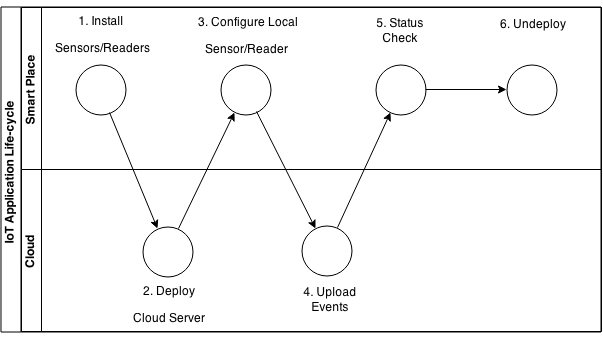
\includegraphics[width=\textwidth]{./images/life-cycle}
  \caption{IoT application life-cycle.}
  \label{fig:life-cycle}
\end{figure}

The life-cycle of an IoT application starts with the installation of the sensors and readers in the smart place (step 1). The next step consists in prepare the
smart place in order to process the events sent by the smart objects. First the application must be deployed at the Cloud in order to be able to receive the events (step 2).
After that the installed sensors and readers must be configured to sent the generated events in the smart place to the application that is running in the Cloud (step 3).
At this point the smart place is already configured to support the processing of events generated by smart objects (step 4). A very important point is to assure that the smart place is working according with the desired Quality of Service (QoS). QoS is a concept that embraces a number of nonfunctional
properties such as price, availability, reliability and reputation \cite{o2002s}. Thus in order to monitoring the performance of the application in the smart place (step 5), these properties
must be agreed between the customer and the service provider, in this case the Cloud provider. This agreement between the customer and the service provider is know as Service Level Agreement (SLA).
The SLA defines the terms and conditions of service quality that a service provider delivers to service requesters based on the \textit{QoS} information \cite{zeng2004qos}.
The final stage that an IoT application can reach is its undeployment, which means that the smart place is deactivated (step 6).\\

Thus, the objective of this work is to decrease the complexity of deployment and management of Cloud-based IoT applications in a smart place.
Usually the deployment of such applications is performed by a technician that manually configure and install the components of the application.
In order to reduce the complexity of this process, the most effective approach is to automate the deployment process of the application. That is achieved
by performing the deployment through Cloud Orchestration tools, that allows to specify the components and the relations between themselves in a high-level
perspective and also provisioning the necessary resources at the Cloud in a effective way. These tools also allows to perform the monitoring of these applications
during its life-cycle as well undeploying them. However, this tools don't solve all our problems. In particular, IoT applications require a software stack that usually
is composed by a database, a web server and the event processing software. But orchestration tools normally lacks the integration of
the event processing software with the other components. Thus, to support the integration of such components these tools must be extend to support the event processing
software.\\

However, managing these applications through a Orchestrator tool requires an elevated technical knowledge. To allow that non-technical users can perform the
managing operations having in perspective the high-level business rules of the smart place, the main objective of this work is to permit that non-technical users
can perform the management of smart places only having in mind the business rules of that particular place. To achieve that, these high-level rules must be translated to
a more low-level rules that can be expressed in terms of non-functional requirements, SLAs, that can be used to estimate the resources needed by the application in order
to have an acceptable \textit{QoS}. In the other hand, to allow those non-technical users to monitoring the smart place, these SLAs must be translated to
a high-level rules that can be expressed in terms of business rules of a given smart place. For instance, if a smart place has a flow of people of 500 persons per day,
that business rule will be translated to a SLA that express the amount of storage and bandwidth required to ensure the \textit{QoS} of the application.
Furthermore, by monitoring the service level offered by the Cloud providers it will be possible to determine if the Cloud is overloaded with the
amount of data generated by the smart place or not.

\NewPage
% -------------------------------------------------------------------------------------------------
% RELATED WORK
% -------------------------------------------------------------------------------------------------
\section{Related Work}
\label{sec:related_work}
Computing infrastructure in location for IoT applications is cost ineffective and presents low scalability.
Recently, the cloud paradigm allowed to move the computing infrastructure to the cloud providers,
making possible to increase the application scalability and also to reduce in a significant way the cost
related with the smart place infrastructure.

% ----------------------------------------
% INTERNET OF THINGS AND CLOUD COMPUTING
% ----------------------------------------
In RFID-based IoT applications, Guinard et al. \cite{guinard2011cloud} point out that the
deployment of RFID applications are cost-intensive mostly because they involve the
deployment of often rather large and heterogeneous distributed systems. As a consequence,
these systems are often only suitable for big corporations and large implementations and
do not fit the limited resources of small to mid-size businesses and small scale applications
both in terms of required skill-set and costs. To address this problem, Guinard et al. propose
a cloud-based solution that integrates virtualization technologies and the architecture of
the Web and its services. The case of study presented in the paper consists of an IoT application
that uses RFID technology to substitute existing Electronic Article Surveillance (EAS) technology,
such as those used in clothing stores to track the products. In this scenario they applied the
Utility Computing blueprint to the software stack - Fosstrak - required by the application using
the Amazon Web Services platform and the Amazon EC2 service. To evaluate the Cloud-based solution,
two prototypes was successfully implemented to prove that the pain points of the RFID applications
can be relaxed by adopting the proposed solution.

However, provisioning applications for Internet of Things still is an issue, because to the Virtual Machines
need to be manually configured and the deployment operation of those applications is specific for each
cloud provider.

% ---------------------------------------------
% AWS
% ---------------------------------------------
Amazon Web Services\footnote{http://aws.amazon.com/} (AWS) offers a variety of services to automate
the provisioning of the IT infrastructure at the Amazon Elastic Computing Cloud (EC2). VM Import/Export is a
service provided by AWS that enables to import virtual machine images from the development environment
to EC2 instances and export them back to the on-premisies development environment. This offering allows
to leverage the existing investments in the virtual machines that was built to meet the IT security,
configuration management, and compliance requirements by bringing those virtual machines into EC2 as
ready-to-use instances. The instances also can be exported to the on-premises virtualization infrastructure,
allowing to deploy workloads across the IT infrastructure. Another service provided by AWS is Elastic Beanstalk
that allows to quickly deploy and manage an application in the AWS cloud. The application is uploaded to AWS,
and Elastic Beanstalk automatically handles the details of capacity provisioning, load balancing,
scaling and application health monitoring. Elastic Beanstalk supports several types of applications,
including Java, Python, Ruby on Rails and Docker containers.

% ---------------------------------------------
% TOSCA
% ---------------------------------------------
TOSCA (Topology and Orchestration Specification for Cloud Applications) \cite{li2013towards} is a new
cloud standard to formally describe the internal topology of application components and the deployment
process of cloud applications. TOSCA is proposed in order to improve the reusability of service management
processes and automate IoT application ratified by OASIS in deployment in heterogeneous environments.
The structure and management of IT services is specified by a meta-model, which consists of
a \textit{Topology Template}, that is responsible for describing the structure of a service, then there
are the \textit{Artifacts}, that describe the files, scripts and software components necessary to be
deployed in order to run the application, and finally the \textit{Plans}, that defined the management process
of creating, deploying and terminating a service. The correct topology and management procedure can be inferred
by a TOSCA environment just by interpreting the topology template, this is known as ``declarative" approach.
Plans realize an ``imperative" approach that explicitly specifies how each management process should be done.
The topology templates, plans and artifacts of an application are packaged in a Cloud Service Archive (.csar file)
and deployed in a TOSCA environment, which is able to interpret the models and perform the specified management
operations. These .csar files are portable across different Cloud providers, which is a great benefit in terms
of deployment flexibility. To demonstrate the feasibility of TOSCA in facilitating IoT application deployment, a typical
application in building automation to control an Air Handling Unit (AHU) was used as scenario. The common IoT
components, such as gateways and drivers will be modeled, and the gateway-specific artifacts that are
necessary for application deployment will also be specified. By archiving the previous specifications
and corresponding artifacts into a .csar file, and deploying it in a TOSCA environment, the deployment
of AHU application onto various gateways can be automated. As a newly established standard to counter
growing complexity and isolation in cloud applications environments, TOSCA is gaining momentum in industrial
adoption as well as academic interest.

\NewPage
\section{Solution Architecture}
\label{sec:solution_architecture}
Actually a typical scenario for an IoT application consists of a smart space that contains several smart objects and all
the infrastructure required to support this application, namelly RIFD tags, sensors, readers and servers, as illustrated at the
Figure \ref{fig:smart-space}. This scenario presents several issues regarding the deployment of the application, the low scalability, the costs of infrastructure
and the maintenance of the same.
% Typical Smart Space Scenario
\begin{figure}[h!]
  \centering
  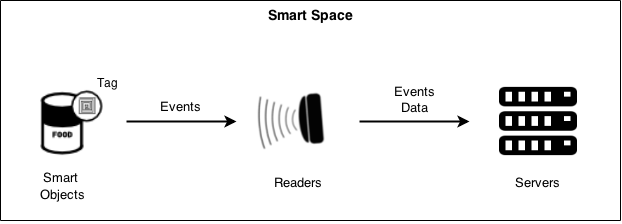
\includegraphics[width=\textwidth]{./images/smart-space}
  \caption{Typical smart space scenario.}
  \label{fig:smart-space}
\end{figure}\\
By converging the IoT applications with the Cloud Computing paradigm the objective is simplify this scenario by leveraging the required infrastructure by these applications to the Cloud providers,
as illustrated at the Figure \ref{fig:smart-space-cloud}. Furthermore, the convergence of this two paradigms, allows to take advantage of the benefits offered by Cloud computing as referenced
in \textbf{Section \ref{sub:cloud_computing}}.
% Cloud-based Smart Space Scenario
\begin{figure}
  \centering
  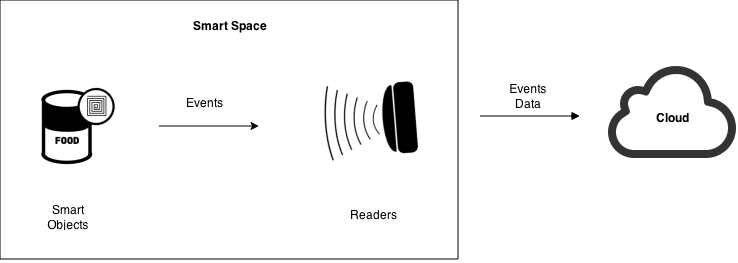
\includegraphics[width=\textwidth]{./images/smart-space-cloud}
  \caption{Cloud-based smart space.}
  \label{fig:smart-space-cloud}
\end{figure}\\
% -----------------------------------------------
% STATE OF ART
% -----------------------------------------------
\subsection{State of Art}
\label{sub:state_of_art}
Actually Cloud-based IoT applications are the state of art of this kind of solutions. By leveraging the infrastructure to the Cloud providers, these applications has a high-availabity, can dinamically scale
while spending a fraction compared with the tradional solutions. However, as earlier mentioned the deployment of such applications still is an issue, due its complexity and required manual intervention. The
deployment of Cloud-based IoT applications usually are performed through IT automation tools, such as Chef\footnote{www.chef.io} and Puppet\footnote{puppetlabs.com}. These tools enables to automate the deployment
of such applications in a certain way, given that all the components of the application and the relation between themselves must be specified manually, which requires considerable manual work and expertise by
the person that is performing the deployment. However, the deployment process of these solutions is not the only existent issue. Monitoring the application life-cycle is a task that requires a lot of effort and expertise
by the system admnistrators.\\

In order to solve this problem, the adopted approach relies on perform the deployment of these applications by using Cloud Orchestrator tools. As mentioned in \textbf{Section \ref{sub:cloud_orchestration}}, these
tools allows to specify the application components and their relations in a high-level perspective and to execute the management tasks required by the application during its life-cycle.
As a matter of fact, in a low-level perspective cloud orchestration tools express the high-level perspective defined by the user into scripts that latter are executed using IT automation tools such as Puppet and Chef.
% -----------------------------------------------
% CLOUD OF THINGS ARCHITECTURE
% -----------------------------------------------
\subsection{Cloud of Things Architecture}
\label{sub:cloud_of_things_architecture}
The main objective of Cloud of Things decrease the complexity of deployment and management of IoT applications. To achieve this objective, Cloud of Things must enable non-technical users - the business managers - to perform the
monitoring of Cloud-based IoT applications as well defining Service Level Agreements in a high-level way. In order execute this tasks, users must be able to interact with the application that is running at the cloud in order
to observe their state and to apply some decisions based on the performance of the application. Thus, Cloud of Things must provide a service that allows the users to perform such actions. At Figure \ref{fig:cloud_of_things_architecture}
we present the Cloud of Things architecture.
\vspace{1in}
% Cloud of Things Architeture
\begin{figure}[h!]
  \centering
  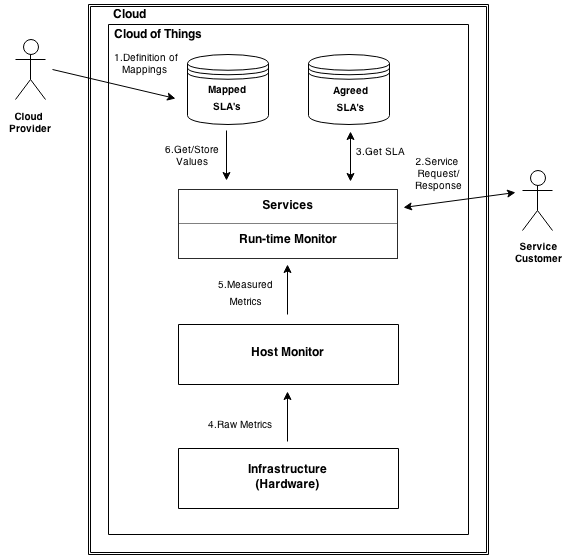
\includegraphics[width=.8\textwidth]{./images/cloud-of-things-architecture}
  \caption{Cloud of Things Architecture.}
  \label{fig:cloud_of_things_architecture}
\end{figure}\\
The presented architecture is based on the LoM2HiS Framework \cite{emeakaroha2010low} architecture. In this architecture the \textit{Services} component and the \textit{Run-time Monitor} represents the application layer where services are
deployed using a Web Service container. The \textit{Run-time Monitor} is responsible to monitor the services based on the negotiated and agreed SLAs. After the Cloud provider agrees on the SLA terms, the agreed SLAs are stored in the repository for
service provisioning and the following steps are executed:
\begin{enumerate}
  \item The Cloud provider creates rules for the framework mappings using Domain Specific Languages\footnote{Domain Specific Languages are small languages that normally are tailored to a specific problem domain.} (DSL's).
  \item The customer requests the provisioning of an agreed service.
  \item Once the request is received, the run-time monitor loads the service SLA from the agreed SLA repository.
  \item The resource metrics are measured by monitoring agents, these metrics are stored in a raw format that later are accessed by the host monitor.
  \item The host monitor extracts metric-value pairs from the raw metrics and them transmits them periodically to the run-time monitor.
  \item After receive the low-level metrics, the run-time monitor uses predefined mapping rules to map the low-level metrics into a equivalent form of the agreed SLA and them the resulting map is stored in the mapped metrics repository.
\end{enumerate}\\
In this architecture, the \textit{Run-time monitor} uses the mapped values to monitor the status of the deployed services. Once it detects that a SLA is violated, the \textit{Run-time monitor} must alert the customer of the violated SLA.
At this point the customer is responsible to take the decisions in order to correct the state of the system.

\NewPage
\section{Evaluation Methodology}
\label{sec:evaluation}
The evaluation of the solution will be performed according to two perspectives: one consists in
evaluating the performance of the Cloud and the other consists in evaluate the performance
of the deployment of the application.
% -------------------------------------
%  APPLICATION DEPLOYMENT EVALUATION
% -------------------------------------
\subsection{Application Deployment Evaluation}
\label{sub:application_deployment_evaluation}
The performance of the application deployment is an important aspect to be evaluated.
The deployment operation can be evaluated in terms of the metrics of \textit{Network Bandwith},
\textit{Data Volume} and \textit{Latency} of the process. These values determine
the efficiency of the deployment operation. For instance, if we have a high \textit{Data Volume}
and a low \textit{Network Bandwith} available, the \textit{Latency} of the deployment process
will present high values.     
% -------------------------------------
%  CLOUD PERFORMANCE EVALUATION
% -------------------------------------
\subsection{Cloud Performance Evaluation}
\label{subs:cloud_performance_evaluation}
An aspect that is important concerns with the performance of the Cloud regarding the amount
of data generated by the events. Cloud computing creates an illusion that available computing
resources on demand are limitless \cite{armbrust2009m}. However, with the increase of the amount of
events, we must measure these computing resources in order to determine if the system is fulfilling
the \textit{QoS} requirements. To perform the evaluation of the behaviour and performance of the Cloud
we need to measure some system metrics such as:
\begin{itemize}
  \item \textit{CPU Utilization:} indicates the percentage of time that the CPU was working at
  the instances in the Cloud. Normally, this metric is available through the Cloud providers.
  Usually, the range of this metrics is given in percentage that can vary between 0-100\%.
  \item \textit{Memory Usage:} indicates the amount of memory that is consumed by the system in a
  given period of time. The unit of this metric is given in MBytes.
  \item \textit{System Load:} is a metric that indicates the general state of the system.
  This metric estimates the general performance of the system by measuring the number of received events.
  The range of this metric varies between 0 and 1. When this metric has a value of 0, it means that the
  system is not receiving any events at the time. If this metric has a value of 1, it means that the system
  is overloaded, consequently the CPU Utilization and Memory Usage metrics are close to the maximum value.
\end{itemize}

\NewPage

%!TEX root = ../dissertation.tex

% Conclusion
\section{Conclusion and Future Work}
\label{sec:conclusion}
The present work explored the deployment of \gls{IoT} applications for smart warehouses based on the
\gls{RFID} technology with two different approaches to deploy: one based in a traditional cloud
deployment approach (cloud-based) and other according the Fog Computing platform (fog-based). More
specifically, the present work focuses to determine if a cloud-based approach is able to meet the
low-latency requirements of many \gls{IoT} applications, since that low-latency is an essential
requirement of \gls{IoT} applications. If a cloud-based approach is not able to meet the network latency
requirements for those applications, the cloud platform is not a viable option to perform the
provisioning of \gls{IoT} applications.

To improve the provisioning of \gls{RFID} middleware in the cloud, we developed a mechanism based on
Docker containers and the Chef tool that automates the installation and configuration of the modules
that composes the Fosstrak platform \gls{RFID} middleware. This mechanism was of extreme
importance, because it allowed us to perform the application provisioning of the cloud instances in
a very efficient way. Although our experiments were conducted in a single cloud provider, the developed
mechanism gave us the flexibility to choose between several cloud providers to provision the
\gls{RFID} middleware.

Regarding the system evaluation, we defined two methodologies for evaluate the latency of an event that
occurs in the physical space and the data storage performance for the Fosstrak platform. With the
methodologies proposed, we were able to compare the event latency performance for both cloud-based
and fog-based approaches. We defined two experiments to evaluate the latency performance of the
deployment approaches. The obtained results shows that the event latency performance presented better
results when the application was deployed according the fog-based approach. However, we identified
some issues regarding the behavior of a Fosstrak module (\gls{ALE}) that affected the performance
of the event latency for both deployment approaches. Regarding the data storage performance of the
RFID middleware, the results show that the Fosstrak platform is able to process with an acceptable
performance the amount of data that is generated in a smart warehouse.

% Future Work
\subsection{Future Work}
\label{sub:future_work}
In the present work, we achieved our initial goals and determine that a fog-based approach is more
adequate to deploy a smart place application based in \gls{RFID} technology. However, our solution
is not perfect and there some aspects that can be improved in the future.

Our solution proposes that the \gls{RFID} application is deployed following a fog-based approach.
This means that we need to have a cloud close to the ground and this cloud must meet the same
requirements of a remote cloud such as high scalability, security and multi-tenancy. Unfortunately,
we were not able to implement a fog that meet these requirements and in our implementation the fog
was built on top of a traditional Virtual Machine. In the future, the fog needs to be correctly
implemented providing all the features of the remote cloud and in addition features such as
location-awareness, mobility support and geo-distribution.

In the current implementation we used Docker containers to provisioning the Fosstrak software stack.
In the evaluation of our solution we deploy the containers in a \gls{EC2} \gls{VM}, which overlays two
different mechanisms of virtualization. Although we still are able to take advantage of some benefits
from the containers such as the portability, other benefits such as the low I/O and disk space are
hidden by the \gls{VM} hypervisor. A future improvement that can be made is to perform the deployment
of the containers on top of the bare-metal or in a cloud-based container service - e.g. Google Kubernetes
\footnote{\url{http://kubernetes.io/}} or \gls{AWS} \gls{EC2} Container Service\footnote{\url{https://aws.amazon.com/ecs/}} -
in order to improve the overall performance of the solution.

Regarding the system evaluation, it was performed only in \gls{AWS} \gls{EC2} instances. For the future
is important to evaluate our solution in other cloud providers to compare which offers the best cost/performance
relation. Also, in experiments performed to evaluate the latency interaction, we defined only two
different \textit{ECspecs}. For the future work, we want to evaluate the latency performance for
our solution with \textit{ECspecs} that presents smaller periods in order to determine which
specification is more suitable for our solution.

In the evaluation scenario we used a virtual RFID reader instead of a physical one, which
does not allow reproducing the environment conditions of a real smart warehouse such as interferences
in the RFID tags antennas, network bandwidth variations, etc. However, in the evaluation experiments
we used for some experiments traces from the work developed by Correia et. al \cite{Correia:Thesis:2014},
which have the real data traces mentioned above. A future improvement is to conduct the system evaluation
in a real scenario in order to have more accurate results.

Finally, the Utility Computing allows to leverage the smart place infrastructure to the cloud,
where the resources are available in a pay-as-you-use model. However, there is a
trade-off between performance and costs. By leveraging the smart place infrastructure
to the cloud, we can reduce the costs of the smart place operation, but the
application performance can be compromised. For the future work, we want to perform
an analysis to establish the relation between the performance and cost of a smart place
regarding its deployment approach: cloud, fog and local. This analysis will allow
to choose which is the most adequate approach to deploy an smart place based in
the performance of the application and the costs of the smart place operation.

\NewPage
\appendix
\section{Planning}
\label{sec:Planning}
In this section we propose a schedule that estimates the required time in future work that will be realized.\\

\bibliographystyle{ieeetr}
\bibliography{../bibliography/references}
\end{document}
